\documentclass{beamer}
\usetheme{metropolis}
\usepackage{subcaption}

% Configuration des couleurs modernes
\definecolor{myblue}{RGB}{173, 216, 230} % Bleu pastel
\definecolor{mymagenta}{RGB}{238, 130, 238} % Magenta doux
\definecolor{mywhite}{RGB}{255, 255, 255} % Blanc pur
\definecolor{mygray}{RGB}{245, 245, 245} % Gris clair
\definecolor{darkblue}{RGB}{25, 25, 112} % Bleu foncé
\definecolor{darkviolet}{RGB}{148, 0, 211} % Violet foncé
\definecolor{goldenrod}{RGB}{218, 165, 32} % Or doux

% Arrière-plan sobre et clair
\usepackage{tikz}

\addtobeamertemplate{background canvas}{}{
	\begin{tikzpicture}[remember picture, overlay]
		\fill[mywhite] (current page.south west) rectangle (current page.north east);
		\begin{scope}[blend mode=overlay]
			\shade[inner color=myblue!60, outer color=mywhite] (current page.south west) rectangle (current page.north east);
			\shade[inner color=mymagenta!60, outer color=mywhite] (current page.north east) rectangle (current page.south west);
		\end{scope}
	\end{tikzpicture}
}

% Personnalisation des couleurs dans metropolis
\setbeamercolor{normal text}{fg=black}
\setbeamercolor{frametitle}{bg=mywhite, fg=black}
\setbeamercolor{title separator}{fg=mymagenta}
\setbeamercolor{progress bar}{fg=myblue, bg=mymagenta}
\setbeamercolor{block title}{bg=myblue, fg=black}
\setbeamercolor{block body}{bg=mywhite, fg=black}
\setbeamercolor{alerted text}{fg=darkviolet!70}

% Personnalisation des typos
\setbeamerfont{frametitle}{size=\Large,series=\bfseries}
\setbeamerfont{title}{size=\Huge,series=\bfseries}

% Apparence des transitions entre les frames
\metroset{progressbar=frametitle,numbering=fraction}

% Commande pour ajuster le séparateur du titre
\metroset{titleformat frame=smallcaps}

% Début du document
\begin{document}
	
	\title{Modèle de Diffusion}
	\subtitle{Machine Learning pour Physicien - Projet}
	\author{Clément, Grégoire, Eliot}
	\date{\today}
	
	\maketitle
	
	\section{Modèle de diffusion}
	
	\begin{frame}{Présentation générale}
		
		Les modèles de diffusion permettent de générer des images distribuées \alert{de la même manière} qu'un dataset donné.
		
		\begin{figure}
			\centering
			\begin{subfigure}[b]{0.4\textwidth}
				\centering
				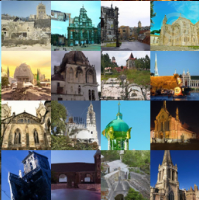
\includegraphics[scale=0.36]{imgs/Church_dataset.png}
				\caption*{Dataset}
			\end{subfigure}
			\begin{subfigure}[b]{0.4\textwidth}
				\centering
				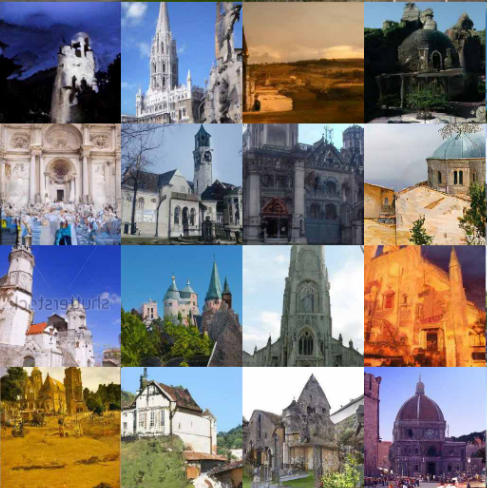
\includegraphics[scale=0.15]{imgs/Church_generated.png}
				\caption*{Images générées}
			\end{subfigure}
			\hfill
			\caption{Source : Denoising Diffusion Probabilistic Models, Ho. and Al.}
		\end{figure}
		
	\end{frame}

 	\begin{frame}{Exemple d'application physique : modèle d'Ising 2D}
        \begin{figure}
            \centering
            \includegraphics[width=0.45\linewidth]{Ising_2D.png}
            \label{fig:enter-label}
        \end{figure}
        \begin{equation*}
            H(\sigma) = -\sum_{\langle i, j \rangle} J_{ij} \sigma_i \sigma_j - \mu \sum_j h_j \sigma_j
        \end{equation*}
        \end{frame}

        
        \begin{frame}{Exemple d'application physique : modèle d'Ising 2D}
        
        A température T, on a $p(\Vec{s}) = \frac{1}{Z} \exp\left(-\frac{E(\Vec{s})}{k_B T}\right)$ \\
        $\implies$ On veut échantillonner des états probables du système \\
        \vspace{0.8cm}
        
        \textbf{But :} Trouver des schémas récurrents d'alignement de spins de matériaux magnétiques, Calculer des grandeurs moyennes caractéristiques... \\
        \vspace{0.8cm}
        \textbf{Méthode :} Metropolis Hasting / Diffusion \\
        $\implies$ Etats discret MH / Etats Continus Diffusion
	\end{frame}

        \begin{frame}{Exemple d'application physique : Débruitage IRM}
        \small Les signaux en physique sont naturellement bruités :
        \begin{figure}
            \centering
            \includegraphics[width=0.46\linewidth]{IRM_bruite.png}
            \caption{IRM avant débruitage}
        \end{figure} \\
        
        \small Utiliser de la diffusion permet de réduire ce bruit pour rendre les photos interprétables :
        \begin{figure}
            \centering
            \includegraphics[width=0.46\linewidth]{IRM_debruite.png}
            \caption{IRM débruité}
            \label{fig:enter-label}
        \end{figure}
        \end{frame}
	
	\section{Denoising Diffusion Probabilistic Models (DDPM), théorie}
	
	\begin{frame}{Idée Générale}
		\only<1>{Considérons un ensemble de \alert{chiffres écrits à la main $D$}. Peut-on trouver une distribution de probabilité $q$ telle que \alert{$x \sim q(x)$ ?}
			\begin{figure}
				\centering
				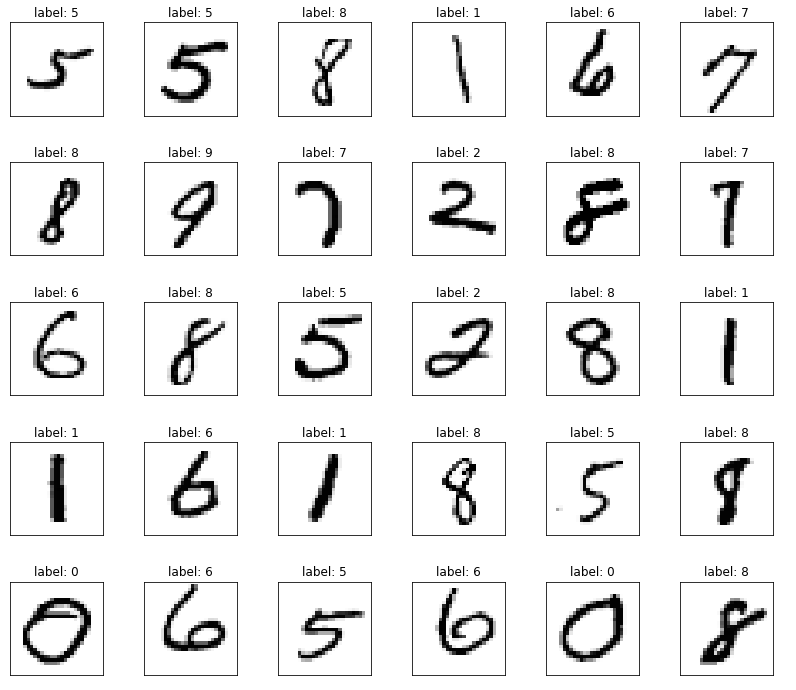
\includegraphics[width=0.5\textwidth]{imgs/mnist_sample_digits.png}
				\caption{Source: ludwig.ai}
			\end{figure}
		}
		\only<2->{
			Considérons l'ensemble de \alert{chiffres écrits à la main $D$}. Est-il difficile de trouver $q$ tel que \alert{$x \sim q(x)$}, nous avons besoin \alert{d'une manière plus intelligente d’échantillonner nos chiffres écrits à la main}. Examinons le procédé suivant:
			\begin{figure}
				\centering
				\begin{minipage}{0.2\textwidth}
					\centering
					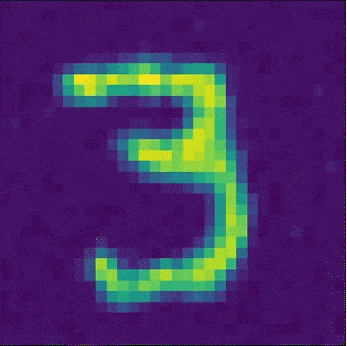
\includegraphics[width=\textwidth]{imgs/frame1.png}
				\end{minipage}%
				\only<3->{
					\begin{minipage}{0.2\textwidth}
						\centering
						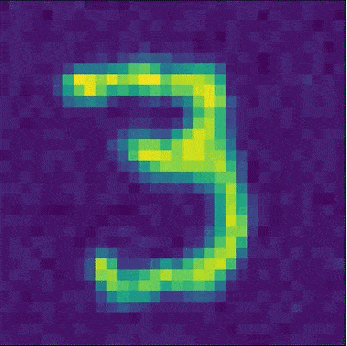
\includegraphics[width=\textwidth]{imgs/frame2.png}
					\end{minipage}
					\only<4->{
						\begin{minipage}{0.2\textwidth}
							\centering
							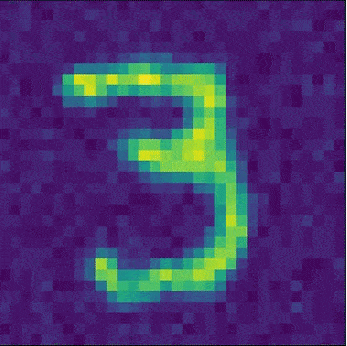
\includegraphics[width=\textwidth]{imgs/frame3.png}
						\end{minipage}
						\only<5->{
							\begin{minipage}{0.2\textwidth}
								\centering
								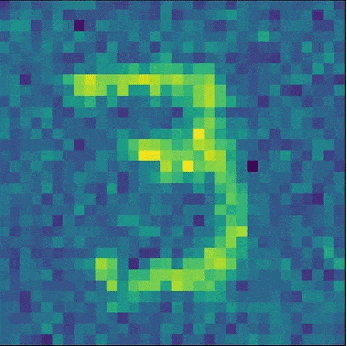
\includegraphics[width=\textwidth]{imgs/frame52.png}
							\end{minipage}
							\only<6->{
								\begin{minipage}{0.2\textwidth}
									\centering
									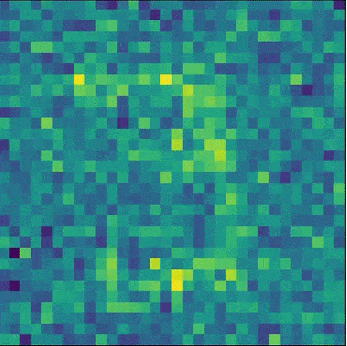
\includegraphics[width=\textwidth]{imgs/framelot.png}
								\end{minipage}
								\only<7->{
									\begin{minipage}{0.2\textwidth}
										\centering
										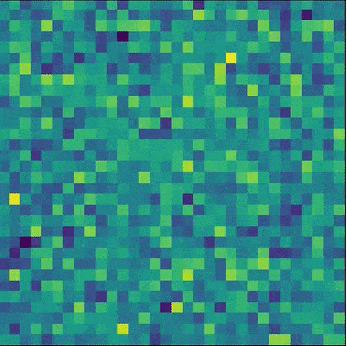
\includegraphics[width=\textwidth]{imgs/framerandom.png}
									\end{minipage}
								}
							}
						}
					}
					
				}
			\end{figure}
			\only<8->{
				Formellement : $q(x_{t+1} \mid x_t) := \mathcal{N}(x_{t+1}; \sqrt{1 - \beta_t} x_t, \beta_t I)$ pour une suite $(\beta_t)_t$. Peut-on \alert{apprendre à renverser ce procédé} ?
			}
		}
	\end{frame}
	
	
	
	\begin{frame}{Que veut-on apprendre}
		En partant d'une image bruitée $x_t$, on \alert{entraîne un modèle pour prédire $x_{t-1}$}.
		\begin{figure}
			\centering
			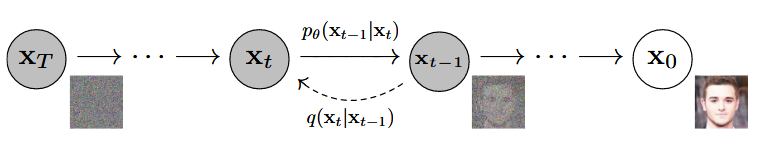
\includegraphics[width= \textwidth]{imgs/ho_diffusion_process.png}
		\end{figure}
		
		\only<2->{
			\begin{itemize}
				\item{En partant d'un set de données \alert{d'images $x_0$}, on échantillonne $(x_t){1:T}$ selon $q(x{1:T} \mid x_0) := \prod_{t=1}^T q(x_t \mid x_{t-1})$,}
				\only<3->{\item{Soit une \alert{image bruitée $x_t$} et $t$, on échantillonne selon $p_\theta (x_{t-1} \mid x_t) := \mathcal{N}(x_{t-1} ; \mu_\theta(x_t,t), \Sigma_\theta (x_t,t))$}.}
			\end{itemize}
		}
	\end{frame}
	
	\begin{frame}{Réduire le coût d'entraînement des données}
		En partant d'une image $x_0$, calculer $x_t$ prend \alert{$t$ échantillonnage sur $q$}. Mais une \alert{astuce simple}, permet de n'en réaliser qu'un.
		\uncover<2->{ 
			
			Rappelons que $q(x_{t+1} \mid x_t) := \mathcal{N}(x_{t+1}; \sqrt{1 - \beta_t} x_t, \beta_t I)$. Posons $\alert{\alpha_t} = 1 - \beta_t$ et $\alert{\bar{\alpha_t}} = \prod_{i=1}^t \alpha_i$.
			\only<3-7>{
				\begin{align}
					x_t &= \sqrt{\alpha_t} x_{t-1} + \sqrt{1 - \alpha_t} \epsilon_{t-1} \nonumber\\
					\uncover<4->{
						&= \sqrt{\alpha_t} \sqrt{\alpha_{t-1}} x_{t-2} + \sqrt{\alpha_t} \sqrt{1 - \alpha_t} \epsilon_{t-1} + \sqrt{1 - \alpha_t} \epsilon_{t-1} \nonumber\\
						\uncover<6->{
							&= \sqrt{\alpha_t \alpha_{t-1}} x_{t-2} + \sqrt{\alpha_t(1 - \alpha_{t-1}) + 1 - \alpha_t} \bar{\epsilon_t} \label{eq:toexplain}\\ 
							\uncover<7->{
								&= \sqrt{\alpha_t \alpha_{t-1}} x_{t-2} + \sqrt{1 - \alpha_t \alpha_{t-1}} \bar{\epsilon_t} \nonumber
							}
						}
					}
				\end{align}
				\uncover<5-7>{Posons $G_1 \sim \mathcal{N}(0,\sigma_1^2 I)$, $G_2 \sim \mathcal{N}(0,\sigma_2^2 I)$ , la somme des deux donne $g_2 \sim \mathcal{N}(0,(\sigma_1^2 + \sigma_2^2) I)$.}
			}
			\only<8>{
				
				On a \alert{$x_t = \sqrt{\bar{\alpha_t}}x_0 + \sqrt{1 - \bar{\alpha_t}} \epsilon$}.
			}
		}
	\end{frame}
	
	\begin{frame}{Entraînement}
		\only<1>{
			Pour l'instant, notre modèle apprend $\mu$ et $\Sigma$, c'est-à-dire qu'on échantillonne selon
			\begin{align*}
				p_\theta (x_{t-1} \mid x_t) := \mathcal{N}(x_{t-1} ; \mu_\theta(x_t,t), \Sigma_\theta (x_t,t))
			\end{align*}
			\alert{Fixer $\Sigma_\theta$} constant donne le même résultat selon le papier, donc :}
		\begin{align*}
			p_\theta (x_{t-1} \mid x_t) := \mathcal{N}(x_{t-1} ; \mu_\theta(x_t,t), \sigma_t I)
		\end{align*}
		\only<2->{
			La probabilité pour notre modèle de générer $x_0$ est $p_\theta (x_0) := \int p_\theta(x_{0:T}) dx_{1:T}$. \only<3->{En utilisant le log-vraisemblance, sous certaines approximations, on cherche à minimiser
				\begin{align*}
					E_q \left[\frac{1}{2 \sigma_t^2} \|\tilde{\mu}t(x_t,x_0) - \mu\theta(x_t,t)\|^2\right]
				\end{align*} où $\tilde{\mu}$ est la moyenne optimale \alert{qui dépend de $x_0$ \only<3>{que nous ne connaissons pas}}. \only<4>{En utilisant $x_t(x_0,\epsilon) = \sqrt{\bar{\alpha_t}} x_0 + \sqrt{1 - \bar{\alpha_t}} \epsilon$ nous \alert{avons une fonction de coût sur laquelle réaliser l'entraînement}.}
			}
		}
		
	\end{frame}
	
	\begin{frame}{Notre premier modèle : Un simple modèle linéaire}
		
		Ici on ajoute un schéma de notre modèle, on parle bien de tout, comment on gère le temps, etc...
		
	\end{frame}
	
	\begin{frame}{Nos résultats - Une gaussienne}
		On a commencé en essayant de \alert{générer des gaussiennes}\only<1>{:
			\begin{figure}
				\centering
				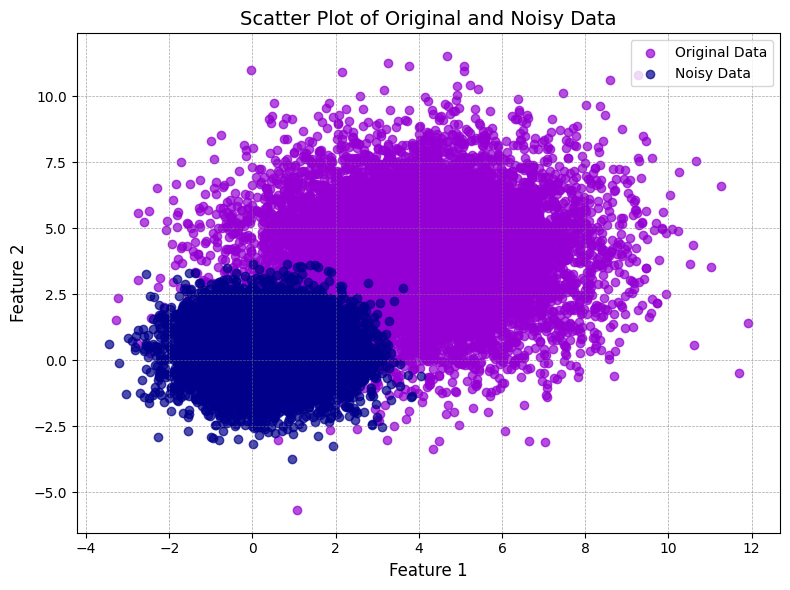
\includegraphics[width= 0.8\textwidth]{imgs/gaussiennes/ho_implementation_init.png}
			\end{figure}
		}\only<2>{ et nous avons eu des résultats encourageants:
			\begin{figure}
				\centering
				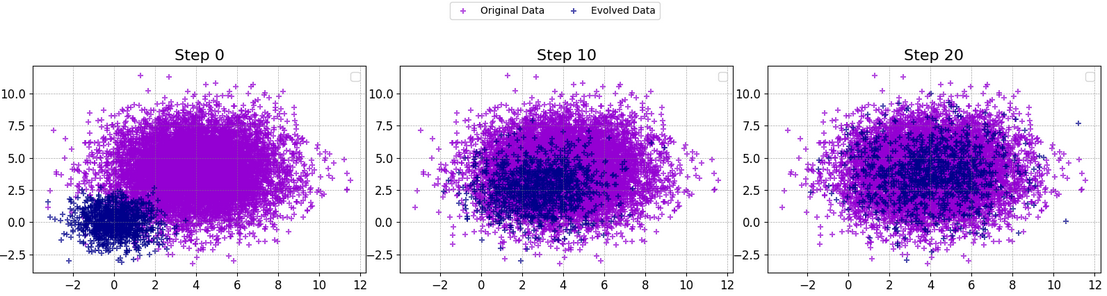
\includegraphics[width= \textwidth]{imgs/gaussiennes/apprentissage.png}
				\vfill
				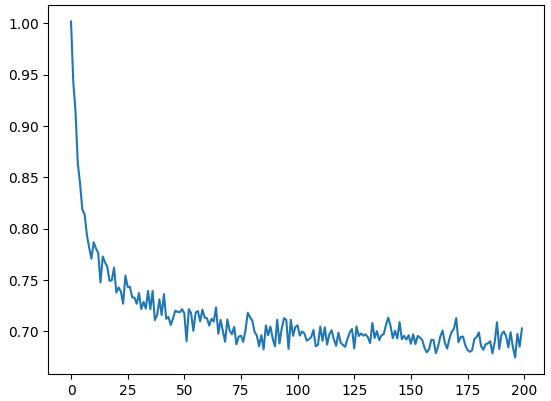
\includegraphics[width=0.4\textwidth]{imgs/gaussiennes/loss.png}
			\end{figure}
		}
	\end{frame}
	
	\begin{frame}{Nos résultats - Deux gaussiennes}
		
		On a ensuite essayé avec deux gaussiennes centrées à des endroits différents \only<1>{
		\begin{figure}
			\centering
			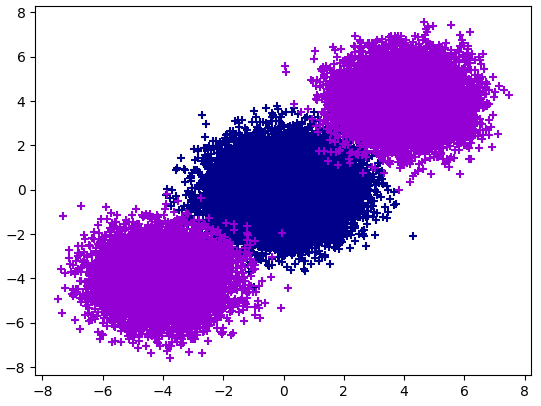
\includegraphics[width=0.7\textwidth]{imgs/deux_gaussiennes/init.png}
		\end{figure} }
		\only<2> {
		\begin{figure}
		\centering
		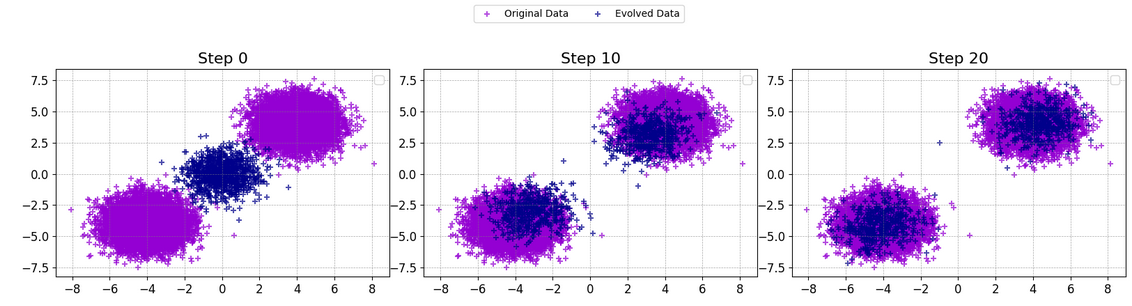
\includegraphics[width=\textwidth]{imgs/deux_gaussiennes/apprentissage.png}
		\vfill
		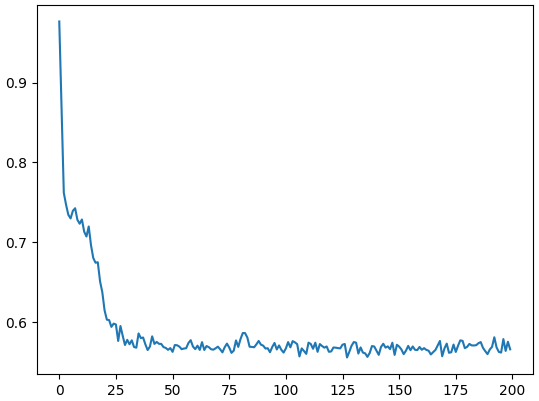
\includegraphics[width=0.4\textwidth]{imgs/deux_gaussiennes/loss.png} 
		\end{figure}}
		
	\end{frame}
	
	\begin{frame}{Nos résultats - Spirale}
		Nous avons ensuite essayé sur un ensemble de données plus compliqué : \alert{la génération de spirale.}\only<1>{:
			\begin{figure}
				\centering
				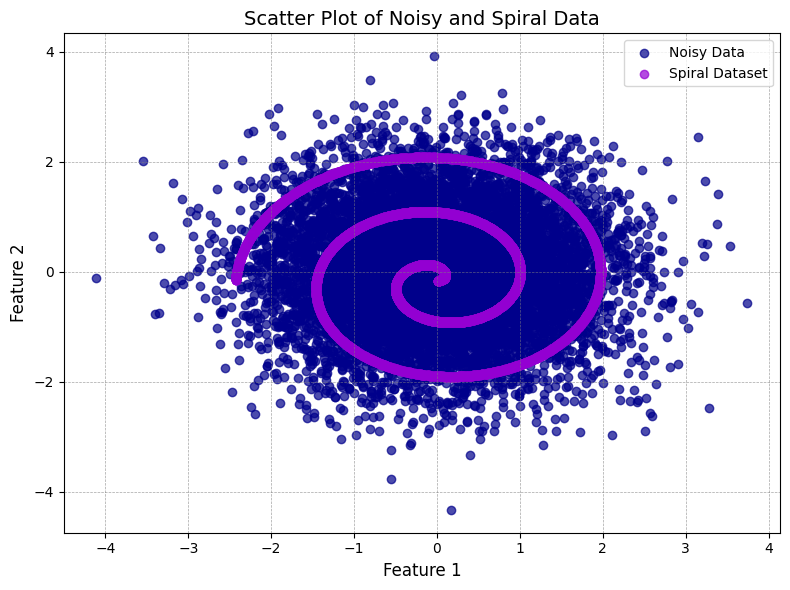
\includegraphics[width= 0.8\textwidth]{imgs/spirales/spirale_dataset.png}
		\end{figure}}\only<2>{ Nous avons également obtenu des résultats satisfaisants :
			\begin{figure}
				\centering
				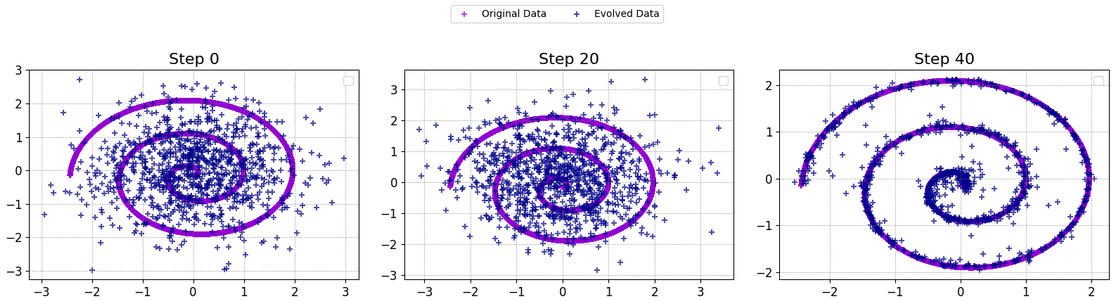
\includegraphics[width=\textwidth]{imgs/spirales/apprentissage.png}
				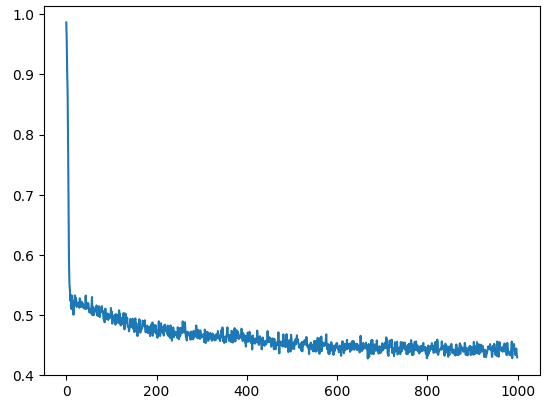
\includegraphics[width=0.4\textwidth]{imgs/spirales/loss.png}
			\end{figure}
		}
		
	\end{frame}
	
	\begin{frame}{Notre deuxième modèle - Un UNet}
		
	\centering \textbf{UNet} : Réseau de neurones spécialisé en traitement d'images \\
        $\rightarrow$ Fonctionne par convolutions successives
        \begin{figure}
            \centering
            \includegraphics[width=0.7\linewidth]{UNet global.png}
            \caption{Structure UNet : Contracting path / Expanding path}
            \label{fig:enter-label}
        \end{figure}
	\end{frame}

        \begin{frame}{Contracting Path}
        \textbf{But :} Capturer des informations précises
        \begin{figure}
            \centering
            \includegraphics[width=1.0\linewidth]{Couches_convolutions.png}
            \caption{Contracting path, première couche}
            \label{fig:enter-label}
        \end{figure} \\
        On applique ensuite un Max pooling pour réduire la résolution.
        \end{frame}

        \begin{frame}{Expanding Path}
        \textbf{But :} Reconstruire l'image en mêlant détails et caractéristiques précises
        \begin{columns}
        \begin{column}{0.5\textwidth}
            \begin{itemize}
                \item On réalise le chemin inverse
                \item Un "Skip connection" permet de rajouter des détails à la reconstruction
            \end{itemize}
        \end{column}
        
        % Colonne de droite : Image
        \begin{column}{0.25\textwidth}
            \includegraphics[width=\textwidth]{UNet expanding.png}
        \end{column}
        \end{columns}
        
        \end{frame}
		
	\end{frame}
	
	\begin{frame}{Nos résultats - MNIST}
		
		
		
	\end{frame}
	
\end{document}
